\documentclass[11pt,a4paper]{article}
\usepackage[a4paper,margin=22mm,headheight=14pt]{geometry}
\usepackage{fontspec}
\setmainfont{texgyretermes-regular.otf}[BoldFont=texgyretermes-bold.otf,ItalicFont=texgyretermes-italic.otf,BoldItalicFont=texgyretermes-bolditalic.otf]
\setsansfont{texgyreheros-regular.otf}[BoldFont=texgyreheros-bold.otf]
\setmonofont{lmmono10-regular.otf}[Scale=0.88]
\ifdefined\chineseversion
  \usepackage[UTF8,fontset=fandol,scheme=plain]{ctex}
  \renewcommand{\abstractname}{摘要}
  \renewcommand{\contentsname}{目录}
  \renewcommand{\refname}{参考文献}
  \renewcommand{\tablename}{表}
  \renewcommand{\figurename}{图}
\fi
\usepackage{amsmath,amssymb,booktabs,tabularx,array,longtable}
\usepackage[table]{xcolor}
\definecolor{inkblue}{HTML}{173B61}
\definecolor{softblue}{HTML}{EFF5FC}
\definecolor{softgreen}{HTML}{EDF5EF}
\definecolor{softgold}{HTML}{FBF3E6}
\usepackage{graphicx,tikz}
\usetikzlibrary{arrows.meta,positioning,fit,calc}
\usepackage{enumitem}
\setlist{nosep,leftmargin=1.5em,topsep=4pt}
\usepackage{titlesec}
\titleformat{\section}{\Large\bfseries\color{inkblue}}{\thesection}{0.6em}{}
\titleformat{\subsection}{\large\bfseries}{\thesubsection}{0.6em}{}
\titleformat{\subsubsection}{\normalsize\bfseries}{\thesubsubsection}{0.6em}{}
\titlespacing*{\section}{0pt}{18pt}{8pt}
\titlespacing*{\subsection}{0pt}{12pt}{5pt}
\titlespacing*{\paragraph}{0pt}{8pt}{0.6em}
\usepackage{caption}
\captionsetup{font=small,labelfont=bf}
\usepackage[section]{placeins}
\usepackage[numbers,sort&compress]{natbib}
\usepackage{xurl}
\usepackage[unicode,colorlinks=true,linkcolor=inkblue,citecolor=inkblue,urlcolor=inkblue,bookmarksnumbered=true]{hyperref}
\usepackage{fancyhdr}
\pagestyle{fancy}
\fancyhf{}
\fancyhead[L]{\small\sffamily Learning to Do Research}
\fancyhead[R]{\small\sffamily Survey / October 2026}
\fancyfoot[C]{\thepage}
\renewcommand{\headrulewidth}{0.3pt}
\setlength{\parindent}{1em}
\setlength{\parskip}{3pt}
\setlength{\emergencystretch}{2em}
\renewcommand{\arraystretch}{1.18}
\setlength{\tabcolsep}{5pt}
\newcolumntype{Y}{>{\raggedright\arraybackslash}X}
\newcolumntype{P}[1]{>{\raggedright\arraybackslash}p{#1}}
\setcounter{tocdepth}{1}
\setcounter{secnumdepth}{3}
\clubpenalty=10000
\widowpenalty=10000
\raggedbottom
\AtBeginDocument{\hypersetup{pdfauthor={Awesome Autoresearch project},pdfsubject={Question-centered survey and proposed research agenda; no new experimental results}}}

\hypersetup{pdftitle={Learning to Do Research: A Question-Centered Survey of AI Research Taste, Discovery, and Experience}}
\title{\textbf{Learning to Do Research}\\[5pt]\Large A Question-Centered Survey of AI Research Taste,\\Discovery, and Experience}
\author{Awesome Autoresearch project}
\date{Literature snapshot: 26 October 2026\\\small Working survey and proposed research agenda}
\begin{document}
\maketitle
\begin{abstract}
AI systems can now propose ideas, modify code, run experiments, and write research reports. The harder question is whether they make better research decisions: choosing useful unknowns, designing informative tests, rejecting weak explanations, and carrying lessons into new projects. This survey organizes 79 resources from the Awesome Autoresearch collection around five questions: research taste, question formulation, reliable execution, learning from experience, and evaluation. It compares the feedback and evidence used by different methods rather than treating workflow completion as a single measure of scientific ability. The collection contains 72 papers, six essays or talks, and one software project. Each question section ends with limitations, open questions, and two concrete experimental directions. We then identify three practical starting projects and a shared evaluation protocol. AI research is the main testbed, with mathematics as a complementary setting. The proposed experiments are research designs, not reported results or claims of established novelty.
\end{abstract}

\noindent\textbf{Keywords:} autoresearch; AI for meta-science; research taste; hypothesis generation; AI scientists; research-agent learning.

\tableofcontents
\clearpage
\section{Scope: improving the research process}
\label{sec:scope}

The central question of this survey is how to build AI systems that become better at doing research. This includes choosing a problem, turning an intuition into a testable claim, obtaining evidence, revising the claim, and improving future decisions. A useful system need not automate every step. A tool that helps a researcher reject an uninformative experiment may contribute more than a pipeline that produces a complete but weak paper.

We use \emph{autoresearch} for this broad methodological direction. It includes human--AI collaboration and autonomous systems. \emph{Meta-science} studies how science works and how its practices can improve. \emph{Meta-learning}, in the narrower machine-learning sense, is one possible technical route to learning research strategies across tasks; it is not a requirement for every method in this collection. Our target is the research process, with AI research as the main experimental setting. We include mathematics because many candidate answers, programs, and constructions can be checked precisely. Checkability helps evaluation, but does not determine whether the question itself matters.

\subsection{Five questions and two timescales}

\begin{figure}[t]
\centering
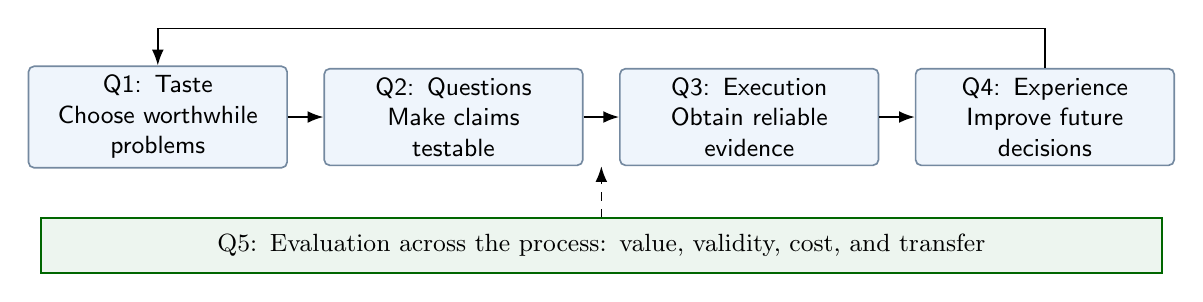
\begin{tikzpicture}[>=Latex,box/.style={draw=inkblue!60,fill=softblue,rounded corners=2pt,align=center,text width=3.05cm,minimum height=1.15cm,font=\small\sffamily},every path/.style={line width=0.6pt}]
\node[box] (taste) {Q1: Taste\\Choose worthwhile\\problems};
\node[box,right=0.45cm of taste] (question) {Q2: Questions\\Make claims\\testable};
\node[box,right=0.45cm of question] (execute) {Q3: Execution\\Obtain reliable\\evidence};
\node[box,right=0.45cm of execute] (learn) {Q4: Experience\\Improve future\\decisions};
\draw[->] (taste)--(question);
\draw[->] (question)--(execute);
\draw[->] (execute)--(learn);
\draw[->] (learn.north)--++(0,0.5)-| (taste.north);
\node[draw=green!40!black,fill=softgreen,align=center,text width=14cm,below=0.65cm of $(question.south)!0.5!(execute.south)$,font=\small,minimum height=0.7cm] (eval) {Q5: Evaluation across the process: value, validity, cost, and transfer};
\draw[dashed,->] (eval.north)--($(question.south)!0.5!(execute.south)$);
\end{tikzpicture}
\caption{The survey's research map. Feedback can revise both the current project and the way later projects are conducted. The ordering is an organizing device, not a mandatory workflow.}
\label{fig:map}
\end{figure}

Q1 asks which problems deserve effort. Q2 asks how to express and develop a question so that investigation can resolve something. Q3 asks whether the system can produce evidence that supports its conclusion. Q4 asks what experience changes in the researcher. Q5 asks how to measure these abilities without confusing one for another. Integrated AI scientist systems are discussed within Q3 because they expose how these components interact.

There are two different timescales. During one project, an agent can improve a candidate solution, revise an experiment, or choose a different search branch. Across projects, it can retain reports, acquire reusable skills, change its control code, or update model weights. A useful conceptual test of the second claim is
\begin{equation}
\Delta_{\mathrm{transfer}} = S(\pi_{\mathrm{after}};\mathcal{T}_{\mathrm{new}},B)-S(\pi_{\mathrm{before}};\mathcal{T}_{\mathrm{new}},B),
\end{equation}
where $\mathcal{T}_{\mathrm{new}}$ contains held-out task families, $B$ is a matched evaluation budget, and $S$ is a declared outcome measure. This is a proposed accounting convention, not a universal definition of scientific progress. The cost of obtaining the experience must also be reported. Better results on the same task used for adaptation do not estimate this transfer quantity.

\subsection{What counts as a good research question?}

A question can be new but unimportant, important but currently untestable, or easy to execute but already answered. We therefore keep five judgments separate: \textbf{importance} of resolving the uncertainty; \textbf{novelty} relative to relevant prior work; \textbf{testability} of the claim; \textbf{tractability} under a stated budget; and \textbf{information value}, including what a negative result would teach. These are our analytic dimensions, not a validated scoring instrument. Their relative importance depends on the field and the purpose of the project.

For example, ``improve this classifier's accuracy'' supplies an optimization target. ``Does the gain from a new augmentation come from invariance or simply from more training updates?'' identifies competing explanations. The second question suggests a matched-compute control and can yield useful knowledge even when the proposed augmentation fails. This example is illustrative; it does not assert that the augmentation question is new. The practical challenge is to make an agent formulate such distinctions using the actual literature and available evidence.

Researchers' essays help articulate the judgment that current benchmarks only partly measure. Olah proposes inexpensive, noisy feedback exercises for developing taste; Karpathy discusses choosing and carrying out projects; Hamming emphasizes the selection of consequential problems~\cite{colah-taste-exercises,karpathy-phd-guide,hamming-you-and-your-research}. Nielsen stresses that good problems often have to be discovered through work, while \emph{Research Debt} explains why better abstractions and explanations can be research contributions~\cite{nielsen-research-heuristics,research-debt}. Nielsen and Qiu place scientific judgment within the institutions that allocate attention and resources~\cite{vision-of-metascience}. These are perspectives and sources of hypotheses for AI research, not experimental evidence that their advice trains effective agents.

\subsection{Corpus and synthesis procedure}

This is a critical narrative survey of a fixed repository snapshot, not a systematic review with an exhaustive search claim. The snapshot contains 72 paper records, six essays or talks, and Karpathy's autoresearch software project. Resources are grouped by their primary contribution in Table~\ref{tab:corpus}. All 79 appear in the discussion and references; some contribute context rather than central empirical evidence. The companion source folder records identifiers, primary URLs, source-review dates, and the citation-to-section coverage.

\begin{table}[t]
\centering\small
\caption{Corpus by primary repository category. Categories overlap conceptually, but resources are counted once.}
\label{tab:corpus}
\begin{tabularx}{\linewidth}{Y r Y r}
\toprule
Category & Count & Category & Count\\
\midrule
Research taste & 8 & Question formulation & 14\\
Research execution & 11 & Learning from experience & 18\\
Evaluation & 16 & Integrated systems & 6\\
Essays and talks & 6 & Total & 79\\
\bottomrule
\end{tabularx}
\end{table}

We compare methods by the decisions assigned to the agent, the human inputs they require, the feedback they consume, and the evidence used to assess success. Core methodological claims are checked against primary papers or official artifacts. Source verification is not independent replication. We avoid pooling headline scores across different model backbones, budgets, task versions, and judging protocols. The proposals at the end of each question section are our research designs. Their sample sizes and resource limits are suggested pilot settings, not power calculations or demonstrated optima. Before claiming novelty for any proposed method, a focused follow-up search is still necessary.

\section{Q1: How can AI judge which research is worth pursuing?}
\label{sec:taste}

Research taste concerns decisions made before their consequences are fully known: which uncertainty deserves attention, which proposal warrants resources, and which result should change the next experiment. A useful evaluator must therefore specify its decision context. Ranking completed papers, selecting untested proposals, and choosing the next experiment are related tasks, but their inputs and available feedback differ. We treat novelty, feasibility, expected information gain, and resource requirements as separate dimensions rather than assuming that one score measures scientific value.

\subsection{What the available feedback actually measures}

AI Can Learn Scientific Taste turns community reception into a training signal. It pairs papers from the same field and year using citation differences, trains a Scientific Judge on these preferences, and uses the judge to reward a Scientific Thinker. Its author, institution, and topic controls address some obvious shortcuts. However, the generator is evaluated through LLM comparisons of potential impact rather than executed projects \cite{ai-can-learn-scientific-taste}. This provides evidence that a preference can be learned and transferred to generation; it leaves the relationship between that preference and realized research value unresolved.

HindSight offers a different target: whether generated ideas resemble subsequent publications, weighted by publication-related impact signals. This makes retrospective comparison possible, but rewards agreement with research that was eventually published. A direction with no later match need not be worthless. More seriously, the reported model knowledge cutoff is later than the retrieval cutoff; restricting retrieved papers alone does not exclude knowledge of the evaluation period \cite{hindsight}. We therefore interpret this as retrospective alignment evidence, not a clean prospective forecast of discovery.

TasteVal moves from paper-level preference to experimental decisions. It supplies a fixed research problem, holds the coding agent constant, and measures progress relative to experimental compute. Its construction helps isolate planning and interpretation from implementation, while making the measured ability conditional on the coder, task, budget, and scoring rule. The tasks are not publicly released \cite{tasteval}. Its results cannot establish open-ended problem selection, and its protocol cannot simply be reused as an available public training set.

Execution can change the judgment itself. The Ideation--Execution Gap study randomly assigns human- or LLM-written ideas within researchers' selected topics, then obtains blinded reviews of the executed projects. The initial advantage of LLM proposals weakens after implementation \cite{ideation-execution-gap}. This is stronger evidence about realized projects than proposal-only ratings, although human execution and a specific NLP setting remain part of the treatment. The studies need not disagree: anticipating community reception, impressing a reviewer, and selecting a productive experiment are different prediction targets.

\begin{table}[t]
\centering
\small
\caption{Feedback for research taste and the inference it permits. None of these targets alone defines scientific value.}
\label{tab:taste-feedback}
\begin{tabularx}{\linewidth}{@{}P{0.22\linewidth}YY@{}}
\toprule
Feedback & Observable target & Remaining uncertainty \\
\midrule
Community reception \cite{ai-can-learn-scientific-taste,hindsight} & Citation preference or later publication alignment & Unpublished alternatives and causal scientific value \\
Expert or grounded judgment \cite{rinobench,opennovelty,innoeval} & Novelty assessments and review agreement & Missing evidence and reviewer preferences \\
Controlled perturbations \cite{scistylebench} & Stability to style and sensitivity to substance & Whether robustness predicts useful research \\
Executed research \cite{tasteval,ideation-execution-gap} & Budgeted progress or post-execution assessment & Dependence on implementation and task selection \\
\bottomrule
\end{tabularx}
\end{table}

\subsection{Evidence-grounded judgment and resistance to shortcuts}

One response is to narrow the judgment and expose its evidence. RINoBench evaluates novelty scores and justifications against expert-review-derived labels. OpenNovelty traces manuscript contribution claims to relevant prior work, while InnoEval combines retrieved evidence with multiple reviewing perspectives \cite{rinobench,opennovelty,innoeval}. These approaches make judgments easier to inspect, but retrieval coverage and the reliability of the comparisons still matter. An apparently convincing rationale can accompany an incorrect score. Moreover, establishing that a claim differs from prior work does not establish that investigating it is worthwhile.

SciStyleBench asks a complementary question: does the judge respond to scientific content or its presentation? Its interventions separate stylistic changes from weakened or enriched substance. The important requirement is joint: scores should resist irrelevant rhetoric while responding to methodological changes. A constant scorer would satisfy invariance without providing useful judgment \cite{scistylebench}. Our synthesis is that evidence grounding and shortcut resistance must be tested together. Adding literature can supply missing facts, but does not automatically make the decision rule faithful to those facts.

\subsection{Limitations and open questions}

Current evidence supports several operational definitions of taste, not a single established capability. Cheap labels permit scale; costly execution gives more direct but narrower feedback. Neither eliminates evaluator disagreement or the need to choose an objective. Open questions include how to credit informative negative results, when a judge should abstain, and whether gains survive new tasks and independent execution. A prospective study should freeze proposals, evaluators, budgets, and accessible knowledge before observing outcomes. The following projects are proposed experiments, not established findings.

\subsection{Proposed project 1: Outcome-grounded ranking with active annotation}

\paragraph{Hypothesis and method.}
At a fixed annotation budget, combining completed pilot outcomes with actively requested expert preferences will select more reproducible, informative projects than learning from proposal ratings alone. Start with a small pairwise judge. Request expert comparisons for uncertain or disagreeing pairs, retain a random annotation fraction, and record selection probabilities. Experts judge completed training pilots using a predefined rubric that credits valid negative results and distinguishes implementation failure from hypothesis rejection.

\paragraph{Tasks and split.}
Construct twelve inexpensive AI research tasks around calibration, retrieval scoring, and robustness of frozen small models. Each task contains six candidate interventions. Assign six tasks to training, three to development, and three to sealed evaluation, grouping shared datasets and code templates together. Run all evaluation candidates with the same coder and budget, with independent replication seeds; their outcomes stay hidden until ranking is frozen. This modest design tests transfer across tasks, not universal scientific taste.

\paragraph{Comparisons, metrics, and risks.}
Compare random selection, a prompted judge, proposal-only preference learning, and outcome-grounded learning with random annotation. Ablate active selection and execution feedback separately. Measure top-$k$ yield of reproducible informative outcomes, ranking regret against the fully executed candidate pool, calibration, annotation cost, and experimental cost. Report uncertainty across tasks. The main risks are noisy outcomes, preference for easy projects, and active sampling that misses unfamiliar ideas; the random fraction provides an audit but does not remove these risks.

\subsection{Proposed project 2: A judge that resists shortcuts without ignoring substance}

\paragraph{Hypothesis and method.}
Separating claims and supporting evidence from presentation cues will improve ranking under stylistic changes without suppressing sensitivity to invalid methods. Build controlled variants of about one hundred proposals: paraphrases, confidence changes, and prestige cues on one side; missing controls, contradictions, or unsupported mechanisms on the other. Independent annotators check whether each transformation preserves or changes the intended content. Train a lightweight pairwise evaluator with both invariance and substance-discrimination objectives.

\paragraph{Tasks, comparisons, and evaluation.}
Split by original proposal, topic, and rewriting model, keeping all variants of an idea in one partition. Compare raw prompting, retrieval-augmented judging, text normalization, and each training objective alone. Measure style-induced score variation, detection of substantive defects, and top-$k$ turnover under adversarial presentation. Also test whether robustness improves selection on the held-out executed tasks from the first project.

\paragraph{Failure risks.}
Rewriting may alter meaning, normalization may erase useful detail, and synthetic defects may be easier than natural research weaknesses. Human audits and untouched proposals are therefore necessary. A reduction in style sensitivity without maintained defect detection or downstream selection quality would count as failure, even if conventional judge-agreement scores improve.

\section{Q2: How can AI formulate useful research questions?}
\label{sec:questions}

A research question identifies something worth resolving; a proposal additionally suggests how to resolve it. Many current systems receive the problem or motivation from a human and generate a new method within that context. Their output can be valuable without demonstrating autonomous problem discovery. For this survey, a useful question should state an unresolved claim, distinguish plausible alternatives, and identify observations that could change the answer. This criterion also makes room for informative negative results, rather than equating research quality with proposing a method that improves a benchmark.

\subsection{Where candidate questions come from}

Literature-grounded systems differ in how they organize the search space. SciMON retrieves inspirations from semantic, knowledge-graph, and citation neighborhoods, then revises ideas against related literature. Its background context already supplies motivations and constraints \cite{scimon}. ResearchAgent develops problems, methods, and experimental plans around a seed paper and connected knowledge; SciPIP combines retrieval with brainstorming; Chain of Ideas organizes prior developments into research trajectories \cite{researchagent,scipip,chain-of-ideas}. These are different priors over possible continuations of existing research. More structured retrieval can improve relevance while also narrowing attention toward well-represented directions.

Broader input does not remove this dependence on representation. MOOSE extracts backgrounds and inspirations from web corpora for social-science hypotheses, whereas SciAgents connects concepts through an ontological graph and specialist agents \cite{moose,sciagents}. Their mechanisms are relevant to general ideation, but judgments of social-science hypotheses and demonstrations in bioinspired materials do not establish transfer to AI research. In particular, a graph connection supplies a candidate analogy, not evidence that the proposed mechanism works.

Data-grounded approaches introduce a feedback loop with a more directly observable target. HypoGeniC maintains natural-language hypotheses, evaluates their predictions on labeled examples, and uses errors and a bandit-inspired rule to guide updates. HypoRefine combines literature-derived hypotheses with this data-driven process, considering both refinement and union of hypothesis sets \cite{hypogenic,hyporefine}. Their classification settings permit held-out prediction tests. This is a useful bridge between verbal claims and observations, but predictive patterns can remain correlational, and the research question is supplied rather than discovered.

\subsection{Human control and the unit of recombination}

Scideator represents papers through purpose, mechanism, and evaluation facets. Users can select facets, inspect novelty evidence, and revise combinations. Its within-subject study compares this representation with paper-level interaction using the same underlying LLM \cite{scideator}. This design provides evidence about the interface and representation, rather than attributing all benefits to a stronger model. It also preserves a role for human judgment when an analogy is unfamiliar or its relevance uncertain.

IdeaSynth similarly supports changing and composing facets through literature-grounded feedback, while CoQuest studies breadth-first and depth-first question development in human-AI interaction \cite{ideasynth,coquest}. These systems suggest that ideation is often an iterative process of reformulating constraints, not merely producing a finished question. However, user control, experienced creativity support, and eventual scientific usefulness are distinct outcomes. A tool that helps a researcher explore more directions has not necessarily learned to choose which direction deserves execution.

\begin{table}[t]
\centering
\small
\caption{Different ideation settings expose different parts of question formation.}
\label{tab:question-settings}
\begin{tabularx}{\linewidth}{@{}P{0.23\linewidth}YY@{}}
\toprule
Setting & Mechanism or evidence & Main unresolved step \\
\midrule
Literature continuation \cite{scimon,researchagent,scipip,chain-of-ideas} & Retrieve and reorganize prior research & Decide whether a new continuation matters \\
Cross-concept hypotheses \cite{moose,sciagents} & Extract inspirations or traverse a graph & Validate the proposed relationship \\
Data-grounded hypotheses \cite{hypogenic,hyporefine} & Update claims using predictive feedback & Move from correlation to an informative question \\
Mixed-initiative ideation \cite{scideator,ideasynth,coquest} & Let users manipulate question components & Separate human selection from system capability \\
Idea benchmarks \cite{ideabench,liveideabench} & Reference contexts or minimal keyword prompts & Connect judged creativity to executable inquiry \\
\bottomrule
\end{tabularx}
\end{table}

\subsection{Generation quality and selection quality are different}

The large human study of NLP ideation finds that LLM proposals can receive favorable novelty judgments while looking weaker on feasibility. Its analysis also identifies repeated ideas as generation scales and unreliable model ranking \cite{llm-novel-research-ideas-human-study}. The implication is conditional: a large candidate pool helps only if it adds useful alternatives and the selector can identify them. Neither property follows from fluent output or a higher sampling temperature.

IdeaBench evaluates generation within reference-paper contexts using model-based comparisons, whereas LiveIdeaBench probes divergent thinking from minimal keyword prompts \cite{ideabench,liveideabench}. Their scores answer different questions because the available context and intended behavior differ. Divergence is valuable during exploration; convergence on a justified, testable question is a separate requirement. Comparisons should therefore hold candidate count, information access, and selection budget constant, and report pool diversity separately from the quality of the selected proposals.

\subsection{Limitations and open questions}

The central gap is between a plausible proposal and an experiment that can resolve uncertainty. Literature novelty checks, user studies, and prediction tests each cover part of this gap, but none alone establishes importance, causal validity, and feasibility together. Open questions include how to discover problems without inheriting their framing, how to recognize meaningful diversity beyond text embeddings, and when to abandon an attractive but untestable idea. Temporal retrieval restrictions also need a model-contamination audit. The following plans are proposed studies; their expected advantages remain hypotheses.

\subsection{Proposed project 1: A proposal paired with a discriminating pilot}

\paragraph{Hypothesis and method.}
Requiring a proposal to include competing explanations and an executable pilot will improve the fraction of projects that resolve a specific uncertainty. The generator must state the central claim, a plausible alternative explanation, predicted observations under each, and a minimal comparison that separates them. For example, a claimed calibration improvement should be distinguished from the effect of additional tuning. A fixed coding agent implements the pilot, and a separate checker audits whether its measurements address the stated alternatives.

\paragraph{Tasks and split.}
Use twelve bounded AI research contexts involving frozen small models: calibration, retrieval scoring, and robustness under controlled input shifts. Reserve six contexts for developing prompts and checking infrastructure, then seal six with disjoint datasets and code-template families. Allow development-set pilot feedback, but freeze the proposed claim and analysis rule before independent evaluation seeds and test examples are revealed. Pilot experiments must not inspect the final test set.

\paragraph{Baselines, metrics, and risks.}
Compare ordinary proposals, proposals with a written experiment plan, and proposals with a discriminating executable pilot. Match total inference and experiment budgets, counting pilot execution against the latter. Ablate competing explanations and the independent checker. Measure executability, blinded assessment of discriminating power, reproducible claim resolution, uncertainty calibration, and cost per informative result. Record inconclusive outcomes separately from implementation errors. Risks include favoring easy questions, underpowered pilots, and a checker that rewards formal compliance; a successful script without a valid discriminating comparison does not count as success.

\subsection{Proposed project 2: Separate exploration from selection}

\paragraph{Hypothesis and method.}
Mechanism-level diversity should improve downstream yield only when paired with a selector that recognizes useful differences. Cross three generators---ordinary sampling, retrieval-based generation, and controlled facet recombination---with random, prompted, and evidence-grounded selection. Each generator produces twenty-four candidates within the same token and retrieval budget. Freeze each pool before applying every selector, so improvements can be attributed to generation, selection, or their interaction rather than to an entire pipeline.

\paragraph{Data, ablations, and measurement.}
Reuse the development and sealed contexts above, with all choices fixed before evaluating held-out pools. Have blinded annotators cluster candidates by substantive mechanism and identify valid alternatives; embeddings serve only as annotation aids. Execute each selector's top three candidates and an independently sampled audit set using the same pilot protocol. Compare candidate count alone, embedding-based deduplication, and facet recombination without a novelty check. Report coverage of valid mechanisms, duplicate burden, top-$k$ informative yield, and cost. Random audits with recorded inclusion probabilities help expose promising candidates that all selectors miss.

\paragraph{Failure risks.}
Mechanism labels can be subjective, and a selector may favor the style of its own generator. Use cross-model selectors, report annotation disagreement, and retain natural candidate wording alongside a normalized evaluation condition. Since only a subset receives execution, avoid claiming an oracle-best pool or exact selection regret. A larger number of textual clusters without increased validated yield would not support the hypothesis.

\section{Q3: How can an agent turn a question into reliable knowledge?}
\label{sec:execution}

Execution connects a research proposal to the world. A program can run successfully while testing the wrong claim. An experiment can improve a metric while leaving the proposed explanation unresolved. A report can accurately describe a selected run while hiding failed attempts. The methodological target is therefore a traceable chain from question to intervention, observation, and appropriately limited conclusion.

\subsection{Search over solutions versus selection of experiments}

Karpathy's autoresearch provides a compact baseline: modify a training program, run a bounded experiment, measure the result, and retain useful changes. AIDE makes branching explicit by searching over executable candidates and deciding when to draft, debug, or improve. R\&D-Agent separates proposing improvements from implementing them~\cite{autoresearch,aide,rd-agent}. These designs make it easier to attribute engineering gains to a search policy. They also show the limitation of using metric improvement as the research objective: the task, metric, and admissible environment are already supplied. A strong optimizer may learn little about why the intervention works.

Arbor organizes hypotheses, artifacts, and experimental evidence in a persistent tree, making branch selection depend on accumulated observations~\cite{arbor}. Its representation is useful for studying research state: which hypothesis is still plausible, which result was reproduced, and which branch has exhausted its budget. The relevant comparison is not simply tree versus linear conversation. It is whether structured state improves a specific decision after matching the number of proposals, trials, and model calls. Its current task setting mainly studies improvement of supplied artifacts and objectives.

AutoRA makes a different decomposition: an experimentalist selects measurements, an experiment runner obtains observations, and a theorist updates a model. Deep Adaptive Design learns a policy for sequential Bayesian experimental design before deployment~\cite{autora,deep-adaptive-design}. These works direct attention to \emph{which observation is useful}, rather than only which implementation scores best. Their assumptions matter: variables, accessible experiments, and model classes or probabilistic assumptions must be specified. Extending information-driven design to open research requires deciding which competing explanations should enter that space.

\subsection{Reliability requires more than successful execution}

Curie checks experiment setup and execution, constrains transitions between agents, and maintains structured experimental records~\cite{curie}. Its distinction between implementation alignment and conclusion correctness is valuable: working code is not enough. The reported evaluation combines automated and human assessment, so its rigor modules should be treated as mechanisms to examine, not a proof that every accepted conclusion is valid.

POPPER targets a supplied natural-language hypothesis through tests of measurable implications and sequential aggregation of evidence~\cite{popper}. Its statistical guarantees depend on the implications and conditional tests being valid. If the experiment tests a different claim, or assumptions fail after adaptive reuse of data, the wrapper cannot repair the scientific error. Error control for one tested hypothesis should also not be presented as false discovery rate control over an unrestricted collection of generated claims. This motivates separating semantic checks, executable controls, and statistical testing in the agent interface.

\begin{table}[tbp]
\centering\small
\caption{Execution mechanisms address different failure points. These are comparisons of design, not a ranking of systems.}
\label{tab:execution}
\begin{tabularx}{\linewidth}{@{}P{0.24\linewidth}YYY@{}}
\toprule
Mechanism / examples & Main decision & Feedback & What remains external\\
\midrule
Code search: autoresearch, AIDE, R\&D-Agent & Which program to try & Measured task score & Task importance; evaluator validity\\
Hypothesis tree: Arbor & Which branch to refine & Artifacts and evidence & Initial objective and evaluation setting\\
Experimental design: AutoRA, DAD & Which observation to obtain & Model fit or information objective & Variables, experiment access, modeling assumptions\\
Process validation: Curie & Whether an experimental step is acceptable & Setup, execution, and record checks & Adequacy of the scientific test\\
Sequential testing: POPPER & Which implication to test & Conditional statistical evidence & Sound implications and test assumptions\\
Program / proof search: FunSearch, AlphaEvolve, Aletheia & Which construction or argument to revise & Evaluator, verifier, or critique & Significance and verification scope\\
\bottomrule
\end{tabularx}
\end{table}

\subsection{What mathematics adds}

FunSearch and AlphaEvolve combine program generation with executable evaluation and evolutionary selection~\cite{funsearch,alphaevolve}. They demonstrate the usefulness of a tight proposal--verification loop when the target admits a precise evaluator. The evaluator is an important human contribution: an agent cannot infer that a fast program is a valid algorithm unless correctness is actually checked. Finite numerical tests, exhaustive verification of a finite construction, and a mathematical proof support different claims.

Aletheia instead iterates mathematical generation, verification, and revision in natural language and reports different degrees of human involvement~\cite{aletheia}. Its outputs should not all be described as formally verified proofs. A useful mathematical extension of our proposed experiments would separate conjecture choice, proof search, and verification. For example, a proof assistant can check a restricted formal statement while human mathematicians judge whether resolving that statement contributes anything. The formal setting gives a validity instrument, not an automatic significance measure.

\subsection{Integrated systems reveal dependencies}

The AI Scientist joins ideation, code, experiments, writing, and review using human-written experiment templates. Version 2 replaces that dependency with a broader experiment manager and agentic tree search, and reports a limited workshop-submission study~\cite{ai-scientist,ai-scientist-v2}. This is evidence about assembling a workflow and producing reviewable artifacts. It does not isolate which component supplies the scientific value or establish general problem-selection ability.

AI-Researcher integrates literature, implementation, and reporting, with Scientist-Bench distinguishing guided innovation from exploration inside research topics. Agent Laboratory makes human-provided ideas and intermediate feedback part of the workflow~\cite{ai-researcher,agent-laboratory}. Human input is an experimental variable, not an inconvenience to omit from a description of autonomy. A fair comparison should record who chose the question, repaired code, interpreted ambiguous findings, and decided to stop.

Co-Scientist evolves hypotheses under scientists' objectives and includes experimental follow-up in biomedical cases. Kosmos uses a structured world model to coordinate literature and data analysis over longer investigations~\cite{co-scientist,kosmos}. Both show why a longer workflow needs persistent scientific state. They also require careful accounting of supplied objectives, data, domain expertise, and external validation. A traceable report is easier to audit; traceability alone does not establish that every claim is correct or important.

The practical lesson is to test interfaces. An idea generator may propose a useful question that its executor cannot implement. An executor may find a result that the writer overstates. Before changing every component, hold the question pool and executor fixed and vary the representation passed between them. A small, well-controlled interface experiment can reveal more than a comparison between two entire systems with different models and budgets.

\subsection{Limitations and open questions}

Most execution evidence concerns supplied objectives with accessible evaluators. It remains unclear whether agents choose experiments that resolve competing explanations, recognize when a result is inconclusive, and preserve that uncertainty in the final report. Existing validators can check declared controls but may miss a missing control. Search over many variants can overfit a validation set even when every individual run is correct. Long investigations also require deciding when to stop, request human input, or change the question. These are research decisions, not merely error-handling tasks.

\subsection{Proposed project I: choosing discriminating experiments}

\paragraph{Untested hypothesis and method.}
Test whether an explicit set of competing explanations improves experimental choices compared with a score-maximizing agent. Represent each question as two or more hypotheses, their predicted outcomes under candidate interventions, and the assumptions required to interpret those outcomes. Select an affordable intervention using disagreement between predicted outcomes or a Bayesian information-gain estimate when a defensible likelihood is available. Preserve an ``undetermined'' option rather than forcing a posterior verdict from an LLM's confidence.

\paragraph{Concrete pilot.}
As an untested design choice, construct eighteen scenarios from six simulator families, with three instances per family, using small tabular models and compact image classifiers. Vary data-generation and evaluation mechanisms, not only random seeds. Allocate two whole families each to construction, development, and testing. Candidate explanations include extra training steps, preprocessing leakage, class imbalance, and useful augmentation. A hidden reference implementation defines the active mechanism or mechanisms. Before agent evaluation, pre-register the allowed interventions and establish which explanations are distinguishable within that simulator and a declared effect tolerance, using counterfactual checks with separate seeds. An injected factor alone is not evidence of unique identifiability. Include coexisting causes, interventionally indistinguishable explanations, and cases where none of the supplied explanations is correct. Permit a set of compatible explanations or abstention when the evidence cannot support a unique answer.

\paragraph{Baselines and measurements.}
Compare the proposed selector with random experiments, a fixed ablation checklist, greedy validation-score search, and an agent without explicit hypothesis bookkeeping. Give all five methods the same intervention access, model, tools, and code-generation module. Measure correct mechanism recovery only on identifiable cases; elsewhere score coverage and excess members of the compatible-explanation set, false explanatory claims, and the error--coverage tradeoff when abstaining. Also record unnecessary experiments and transfer across scenario families. Ablate the hypothesis set, prediction table, and outcome-update rule on development cases. Freeze the oracle, prompts, and stopping rules before testing.

\paragraph{Budget and accounting.}
Run three seeds on each of the six test scenarios. Five methods therefore require ninety target runs. Each run may execute at most four interventions within fifteen worker-minutes of experimental computation, using a declared four-core CPU worker with 16 GB RAM and, for image tasks, at most one 24 GB GPU. The target ceiling is 22.5 worker-hours, at most ninety CPU core-hours, and at most 22.5 GPU-hours if a GPU remains allocated throughout every run; actual CPU and GPU use must be reported separately. Cap simulator/oracle construction and development at ten additional worker-hours each. Remote model computation is outside these device ceilings: allow at most 40,000 input and 8,000 output tokens per target run and record API cost separately. Count failed and truncated trials, oracle checks, and development ablations; never discard them from the ledger because they produced no useful result. These are pilot limits, not measured requirements or a power calculation.

\paragraph{Failure risks.}
A synthetic world may make explanations too clean or give away the mechanism through simulator artifacts. Keep reference code and mechanism labels hidden, publish the simulator assumptions, and inspect whether success survives held-out generators. The six test scenarios occupy only two families, so uncertainty and transfer claims must reflect that small number of independent groups. Improvement here would justify a diagnostic benchmark, not general scientific reasoning. The next milestone would be blinded review of whether the selected controls help resolve real replication disputes.

\subsection{Proposed project II: claim-to-evidence checking}

\paragraph{Untested hypothesis and method.}
Test whether a structured claim ledger reduces unsupported conclusions. Each claim must point to an exact run identifier, code version, data split, reported statistic, and the control needed to support it. A deterministic checker verifies that artifacts and values agree. A separate critic checks whether the experiment distinguishes the asserted explanation. The critic may mark a claim unsupported or inconclusive; it should not edit experimental outputs to make them fit.

\paragraph{Data, controls, and evaluation.}
Propose a pilot with twenty-four completed investigations from twelve parent tasks, two traces per task, drawn from project I or compatible public traces with inspectable provenance. Assign six parent tasks to development and six to testing, keeping related generator families in the same partition. Select five original claims per investigation and construct one perturbed counterpart for each: alter a number, omit a control, confuse validation with test results, or strengthen a conclusion. This yields at most 240 fixed claims, 120 per partition. Two blinded reviewers label each as supported, unsupported, or inconclusive and adjudicate disagreements; a perturbation is not automatically an invalid claim. Keep untouched naturally occurring errors and uncertainty cases in the sample.

For the checking experiment, freeze both the experimental artifacts and this exact claim set. Compare accept-all/no-check, a prompt-only critic, deterministic checks alone, and the combined ledger. All methods receive the same available evidence and return a decision for every claim, so unsupported-claim detection and false-rejection denominators are shared. Report precision and recall, retention of supported claims, and treatment of inconclusive cases separately. Keep every original claim, its perturbation, and its source investigation in the same partition; uncertainty should be clustered by parent task rather than treating sentences as independent.

\paragraph{Attribution and cost.}
Run a separate writer study on the twelve held-out investigations, comparing an ordinary writer with ledger-guided writing. Keep experiments fixed and define the same independently annotated inventory of supportable claims for both writers. Measure supported content covered and unsupported assertions introduced; do not compare their detection scores when they generate different claims. This distinguishes checking from generation and prevents silence from receiving full credit. Any later study allowing checker-requested experiments would test investigation improvement separately.

Use three stochastic replicates per checking or writing condition. Four checking methods over twelve investigations give 144 bundles; cap local artifact processing at five CPU worker-minutes per bundle, or twelve worker-hours. Two writers produce seventy-two reports under the same per-report cap, adding six worker-hours. Permit one independent rerun per held-out investigation, with a fifteen-minute cap each, adding at most three worker-hours and, if required, three GPU-hours. One development replicate per checking and writing condition adds a six-worker-hour ceiling. On the same four-core hardware, the complete local pilot is therefore capped at twenty-seven worker-hours and at most 108 CPU core-hours; remote language-model work is recorded separately, with 40,000 input and 8,000 output tokens per checking bundle or generated report. Report annotation labor, model calls, missing artifacts, and rerun failures alongside costs. Tool failures and critic errors are not evidence that the scientific hypothesis is false, and repeated use of the same parent task does not increase the number of independent tasks.

\section{Q4: How can research experience improve the researcher?}
\label{sec:learning}

A research system can improve its current solution without becoming better at conducting the next investigation. Q4 concerns this distinction: which information survives an investigation, what component it changes, and whether the change benefits subsequent decisions. We separate \emph{within-task adaptation}, reuse across runs on related tasks, and transfer to held-out task families. These are evaluation settings, not interchangeable descriptions of learning. A persistent database can support the second without demonstrating the third; updating model weights during one problem can still be entirely task-local. Research taste requires an additional test of which questions deserve attention, beyond solving assigned problems more efficiently.

\subsection{External memory, reusable skills, and local reflection}

AgentRxiv makes research reports available to later laboratories, while Agora represents shared hypotheses, results, and verifications through Git-based records~\cite{agentrxiv,agora}. Both treat research as an accumulating collective process. Their distinction from an ordinary conversation history is persistence and reuse across sessions. However, persistence alone does not identify the causal contribution of memory: later agents may receive better candidate solutions, more cumulative computation, or more informative task-specific evidence. Agora explicitly leaves discovery gains per unit of computation to matched comparisons.

EvoScientist separates ideation memory from experimentation memory, distilling prior trajectories into directions and implementation strategies. InternAgent-1.5 combines procedural strategies, within-trajectory episodes, and semantic knowledge accumulated across sessions~\cite{evoscientist,internagent-1-5}. These architectures suggest that a research memory should distinguish \emph{what happened}, \emph{why an action was selected}, and \emph{when a lesson applies}. This distinction is our design interpretation, rather than a demonstrated universal memory schema. AutoResearchClaw emphasizes lessons extracted from previous failures; its cross-run ablation primarily supports avoiding known failure modes rather than raising the scientific-quality ceiling~\cite{autoresearchclaw}.

Reusable skills go beyond storing a report by prescribing actions under recognizable conditions. HypoForge refines hypothesis-generation and testing skills using comparative critique and execution feedback, then evaluates them on held-out tasks without updating the backbone~\cite{hypoforge}. This is a useful form of strategy adaptation, but its test-pass metric includes significance for reference hypotheses; it does not independently establish false-positive control or question importance. A skill can learn how to satisfy an evaluator while remaining a poor guide to informative science.

Local feedback must also retain its own category. Reflexion stores verbal reflections without weight updates; Dolphin feeds experimental analysis into subsequent iterations; OR-Agent uses hierarchical reflections and backtracking during heuristic search~\cite{reflexion,dolphin,or-agent}. These methods motivate feedback-sensitive researchers, but their respective evidence should not be rewritten as general cross-task scientific learning. In particular, OR-Agent's verbal gradient and momentum terminology describes an analogy for reflection, not gradient updates to the language model.

\subsection{Changing the research program or training the model}

Code evolution changes the procedure that produces future actions. ADAS searches agent programs using an archive of designs and evaluations; Darwin G\"odel Machine maintains evolving coding agents that modify their own implementations~\cite{adas,darwin-godel-machine}. They are foundations for research-agent design, with evidence from specified benchmark tasks rather than scientific agenda selection. Bilevel Autoresearch makes the inner research loop itself the optimization target: an outer process analyzes traces and generates mechanisms that modify search~\cite{bilevel-autoresearch}. Its reported study concerns one small GPT-pretraining setting. It demonstrates a bounded outer-to-inner intervention, not unbounded recursive improvement or general transfer between research domains.

Parameter training changes the model that proposes or evaluates decisions. CycleResearcher uses an automated reviewer for iterative preference training of research generation~\cite{cycleresearcher}. Its core evaluation includes model-generated experimental results that were not executed; an appendix separately illustrates integration with execution. Consequently, improved manuscript or reviewer scores must not be interpreted as improved empirical discovery. The distinction matters for training data: a fluent retrospective explanation is not necessarily a record of an experiment that happened.

ResearchTrails extracts decision sequences from human Git histories and studies demonstrations, distilled skills, supervised learning, and reinforcement learning~\cite{researchtrails}. Its principal prediction target is the recorded next research decision. Commit histories provide incomplete evidence about human exploration, and similarity to a historical decision does not establish that an alternative policy would discover more. SciSense instead synthesizes citation-conditioned sensemaking trajectories, including reconstructions of paths toward known contributions, and distills them into planning models~\cite{scisense}. Such reconstructions offer structured supervision, but they are not observations of the authors' actual deliberations. Its downstream execution study and judgment-based evaluations remain narrower than general scientific value.

MLE-Ideator provides a more direct execution signal: an ideation model learns strategic guidance through reinforcement learning while a separate agent implements suggestions~\cite{mle-ideator}. Held-out MLE tasks test whether that guidance transfers, but objectives remain supplied. TTT-Discover updates model weights during search on a single problem, whereas Evolution Fine-Tuning trains on evolutionary trajectories before evaluation on held-out optimization tasks~\cite{ttt-discover,evolution-fine-tuning}. This contrast separates task-local adaptation from accumulated cross-task training. EFT's supplied objectives and predominantly shared search scaffold still limit what can be inferred about unfamiliar research workflows or taste.

\begin{table}[tb]
\centering
\small
\caption{What changes through experience? Mechanism and transfer are separate questions; representative works may use several mechanisms.}
\label{tab:learning-mechanisms}
\begin{tabularx}{\linewidth}{@{}P{0.18\linewidth}YY@{}}
\toprule
Mechanism & Changed object and temporal scope & Representative works \\
\midrule
Local reflection & Context and action selection during an investigation & Reflexion; Dolphin; OR-Agent \\
Memory and skills & External evidence or procedures reused in later sessions & AgentRxiv; Agora; EvoScientist; InternAgent-1.5; AutoResearchClaw; HypoForge \\
Program evolution & Controller code or research-loop strategy & ADAS; Darwin G\"odel Machine; Bilevel Autoresearch \\
Parameter training & Model weights, before or during a task & CycleResearcher; ResearchTrails; SciSense; MLE-Ideator; TTT-Discover; EFT \\
\bottomrule
\end{tabularx}
\end{table}

\subsection{Limits of current evidence and open questions}

Across these mechanisms, the central unresolved issue is attribution. A stronger final artifact may reflect additional attempts, retrieved solutions, a better implementer, or a better decision policy. Evaluation should therefore state what is retained, freeze the execution interface where possible, and compare both equal online budgets and total costs including experience collection. Resetting memory or weights between tasks must be explicit. Splitting individual trajectories is insufficient when training and test records share datasets, repositories, or near-identical task templates.

Three questions follow. Which experience preserves reasons and applicability conditions rather than copying successful answers? Can a researcher revise a previously useful strategy when the environment changes? Can learning improve the selection of informative experiments and stopping decisions, even when the final benchmark score does not improve? Answering these requires executed outcomes and independent checks, not only a judge that also supplies the training reward. The following pilots are proposed designs, not reported results; their task counts and budgets are deliberately modest starting assumptions.

\subsection{Proposed pilot A: the causal value of research memory}

\paragraph{Hypothesis and method.}
Structured decision records combining successful and unsuccessful attempts improve subsequent experimental choices more reliably than polished prose summaries. Create a fixed archive with states, proposed actions, stated reasons, observed outcomes, and unresolved uncertainties. Distinguish implementation errors, inconclusive measurements, and evidence against a hypothesis; do not collapse all three into failure. Render the same archive as prose or structured records, retaining provenance links. Freeze the archive before target evaluation so treatments cannot contaminate one another.

\paragraph{Data, splits, and controls.}
As a pilot design, select twelve small public-data ML tasks from tabular prediction, image classification, and compact language-model training. Allocate two tasks per family to archive construction, one to development, and one to a hidden target set; keep underlying datasets and data splits disjoint across these roles. Pre-register task identities after an execution smoke test. Randomize six conditions on the same target tasks and seeds: no memory, full prose summaries, success-only records, failure-only records, combined decision records, and task-shuffled combined records. The prose and combined-record comparison uses the same underlying evidence; success/failure comparisons isolate content. Match retrieval policy and memory-token limits across nonempty conditions. Shuffle task-to-memory associations rather than record order, preserving counts and lengths, to probe whether relevant experience matters.

\paragraph{Metrics and resource accounting.}
Use three seeds per target task. Record the independently checked test outcome of the final artifact selected on validation data, repeated-failure rate, redundant experiments, invalid conclusions, and time to a pre-specified validation improvement. A blinded audit of sampled decision logs checks whether selected experiments address the stated uncertainty. Cap each run at six experiments and 45 minutes of task computation on the same declared hardware: the main target comparison permits at most 40.5 device-hours if every run uses one device throughout. Two archive runs per source task and one development run per task and condition add ceilings of nine and 13.5 device-hours, respectively. Count summarization, retrieval, model tokens, and failed executions separately; also report actual utilization and API cost. These ceilings exclude remote model computation, which must remain in the cost ledger.

\paragraph{Failure risks.}
Task similarity could make retrieval an answer cache; outcome labels could incorrectly turn low power into a negative finding; long records could help through extra context alone. Shuffled-memory controls, provenance inspection, and matched evidence address parts of these risks. With only three target tasks, intervals should be grouped by task and treated as exploratory. A null effect would be informative if it separates useful failure prevention from improved research decisions.

\subsection{Proposed pilot B: distilling strategy across task families}

\paragraph{Hypothesis and method.}
Training on decision states, alternative actions, observed outcomes, and applicability conditions transfers better than imitating next actions alone. Use a fixed implementation agent and evaluator throughout; only the strategist changes. Start with a small open model and parameter-efficient supervised fine-tuning, postponing reinforcement learning until the supervision itself shows a benefit. Require every training outcome to link to an executed log. Unexecuted synthetic rationales may be retained as annotations, but never as observations or evidence that an action succeeded.

\paragraph{Data, splits, and comparisons.}
Propose sixteen tasks, four in each of four families: tabular prediction, image classification, compact language-model training, and numerical algorithm optimization. Reserve whole families, using two for training, one for development, and one for testing. Within every task, keep model-fitting data separate from validation feedback and a sealed final evaluator. The initial pilot uses one pre-registered family split; further rotations would be needed for a general transfer claim. Collect up to six short trajectories per training task, with four experimental decisions each, giving at most 192 executed decision transitions. Compare the base strategist, base plus retrieval from the same archive, action-only fine-tuning, and full decision-context fine-tuning. Use identical source transitions and optimizer-step budgets, report token counts, and add a token-matched development comparison; remove outcomes or applicability conditions in further development ablations.

\paragraph{Metrics, cost, and interpretation.}
Freeze all learned components on the held-out family. Evaluate four target tasks with three seeds, at most four experiments and 30 minutes per run, giving a 24 device-hour ceiling for the four-way target comparison under single-device execution. Set an initial fine-tuning cap of eight device-hours on declared hardware; report teacher trajectories, filtering, development, training, and inference costs separately, alongside performance after amortizing those costs over different numbers of future tasks. Primary outcomes are independently checked task improvement and improvement per total budget; secondary outcomes include invalid experiments, premature stopping, and sensitivity to a changed evaluator interface. Few training examples, family-specific conventions, and contamination can all mimic or hide transfer. Even a positive result would support reusable experimentation strategy under supplied objectives, not autonomous selection of important research questions.

\section{Q5: How should better research be evaluated?}
\label{sec:evaluation}

Evaluating an AI researcher requires specifying which decisions belong to the agent and which are supplied by the evaluator. A correct answer, an improved model, a reproduced result, and a worthwhile research question are different achievements. The evaluation literature provides instruments for parts of this process, rather than a common scale of scientific ability. We organize these instruments by their inputs, decision freedoms, and verification procedures, then propose protocols connecting question quality to subsequent evidence.

\subsection{What existing evaluations actually measure}

MLAgentBench makes experimentation observable through file operations, code execution, and iterative model improvement. MLE-bench situates such behavior in Kaggle-derived prediction tasks, while MLGym supports varied task environments and research artifacts, including algorithmic settings. Their common strength is an executable feedback loop; their common boundary is that the task and success criterion are provided. MLGym explicitly distinguishes its baseline-improvement benchmark from more ambitious research capabilities. AIRS-Bench removes supplied baseline code and uses paper-derived tasks, increasing implementation freedom while retaining a specified problem, dataset, and metric. These changes alter the difficulty and scope of execution without making question selection autonomous \cite{mlagentbench,mle-bench,mlgym,airs-bench}.

RE-Bench adds expert human attempts and comparisons across allocations of time and repeated attempts. It shows why a performance claim must identify its resource regime rather than compare isolated headline scores. FML-bench instead controls the editing and execution infrastructure to isolate decisions about what to try next, separates validation feedback from final held-out testing, and records search behavior. Its experimental-step budget does not equalize all deliberation costs: additional reasoning calls can still consume resources. Together these designs separate engineering infrastructure, research strategy, and computational opportunity \cite{re-bench,fml-bench}.

Reproduction offers another measurable target. CORE-Bench starts from existing computational artifacts: its easy setting supplies outputs, whereas harder settings require increasingly substantial environment setup and execution. PaperBench starts from a paper and clarifications, requiring an implementation assessed through distinct code-development, execution, and result-matching requirements. Its Code-Dev variant omits the reproduction step and therefore supports a narrower inference. PaperBench also evaluates its automated judge against human labels. Reproducing an artifact and independently implementing a paper are complementary capabilities, neither of which establishes the value of a newly selected question \cite{core-bench,paperbench}.

ScienceAgentBench distinguishes successful execution from satisfying a scientific task's output requirements; its checks include task-dependent criteria rather than a universal definition of discovery. SciCode tests scientific knowledge expressed as working programs, with subproblem structure and evaluation settings that vary the supplied background or intermediate solutions. DiscoveryBench moves toward hypothesis content by comparing facets of a discovered relationship with reference findings. These benchmarks respectively emphasize workflow reliability, scientific coding, and recovery of data-supported findings, while retaining externally specified tasks or discovery goals \cite{scienceagentbench,scicode,discoverybench}.

Interactive environments expose investigation itself. ScienceWorld tests grounded experimentation in elementary science; DiscoveryWorld separately assesses task completion, relevant procedures, and explanatory knowledge, with reference-based grading for the latter. Their controlled worlds enable inspection of interventions, but transfer to real research remains a further question. FrontierMath provides difficult mathematical problems with automatically checked answers; the original benchmark does not require formally verified proofs or agent-selected conjectures. Verifiability makes these environments useful, but does not make their scores measures of scientific significance \cite{scienceworld,discoveryworld,frontiermath}.

MLR-Bench broadens the output to ideas, proposals, experiments, and papers within supplied research topics, using structured review rubrics. This exposes qualities missed by prediction accuracy, while making judge calibration and independent verification essential. Many AI Analysts, One Dataset provides a complementary methodological study: with data, hypothesis, and estimand fixed, different model and persona conditions produce different analytical paths and conclusions. Its AI auditor filters methodological failures, but neither exhaustively represents defensible human analyses nor certifies every retained result. Research quality therefore depends on the analysis and evaluation procedures as well as the final report \cite{mlr-bench,many-ai-analysts-one-dataset}.

\begin{table}[tbp]
\centering
\small
\setlength{\tabcolsep}{3pt}
\renewcommand{\arraystretch}{1.15}
\begin{tabularx}{\linewidth}{@{}P{0.20\linewidth}YYYY@{}}
\toprule
Evaluation family & Supplied & Agent chooses & Checked & Still missing \\
\midrule
MLAgentBench; MLE-bench; MLGym; AIRS-Bench & Task, data, metric; starting code varies & Models, code, experiments & Task performance & Question value \\
RE-Bench; FML-bench & Bounded task and starting solution & Improvements and search & Scores and process & Agenda selection \\
CORE-Bench; PaperBench & Artifacts or target paper & Setup or implementation & Outputs or replication requirements & New contribution \\
ScienceAgentBench; SciCode & Scientific task and inputs & Program and analysis & Execution and task tests & Problem significance \\
DiscoveryBench; MLR-Bench & Discovery goal/data or topic & Hypothesis or research plan & Reference facets or review rubric & Independently established value \\
ScienceWorld; DiscoveryWorld & Simulated world and task & Actions and experiments & Task/process; explanations in DiscoveryWorld & Real-world transfer \\
FrontierMath & Mathematical problem & Reasoning and computation & Submitted answer & Proof and conjecture selection \\
Many AI Analysts & Data, hypothesis, estimand & Analytical specification & Audited outcome variation & Exhaustive validity \\
\bottomrule
\end{tabularx}
\caption{Decision and evidence boundaries of the evaluation literature. Grouped rows summarize related instruments, not interchangeable protocols; Many AI Analysts is an empirical study rather than a benchmark.}
\label{tab:evaluation-boundaries}
\end{table}

\subsection{From scores to defensible comparisons}

We recommend reporting a profile: question value, methodological validity, execution success, reproducibility, generalization, and resource use. A scalar aggregate can be supplementary, with its weights declared. Judge agreement should be measured on held-out human annotations, including disagreements and false acceptance of unsupported claims; apparent agreement is not ground truth. Comparisons should fix model access, retrieval conditions, available data, and stopping rules, while separately reporting inference tokens, experiment compute, wall time, parallelism, and human assistance. Every attempted run belongs in the accounting. A best-of-many result must include selection costs, and validation-guided selection must remain separate from final testing. Versioned tasks, evaluators, environments, and archived traces make these claims inspectable.

\subsection{Limitations and open questions}

These instruments leave a central gap: a benchmark can measure progress on a valuable task after humans have already selected it. Reference-based scoring may reject valid unexpected findings, while open-ended reviewing can reward persuasive presentation. Public tasks can overlap with pretraining or retrieval material; fresh tasks reduce observable exposure without proving training independence. Scientific value may emerge only after later reuse, and negative findings can be informative without improving a predictive metric. The unresolved question is how to measure these properties prospectively while maintaining affordable, repeatable comparisons.

\subsection{Proposed project I: prospective idea-to-result evaluation}

\paragraph{Untested proposal and design.}
Build a prospective AI-research benchmark with separate generation and selection tracks. Before outcomes exist, preregister broad briefs, eligibility rules, budgets, and a rubric for importance, novelty, testability, and evidential quality. Obtain human and AI candidate questions under equal quotas, then freeze their text and provenance. All selectors rank the same frozen pool; the generation track separately evaluates which candidates each generator contributes. This prevents better execution or a favorable candidate pool from being mistaken for better selection.

\paragraph{Splits and controls.}
Separate development and test sets by research topic and dataset/code lineage, with a final prospective cohort collected after agent development. Keep experimental test data hidden and freeze literature snapshots, logging all subsequent retrieval. Baselines should include random selection, a fixed novelty/feasibility heuristic, a one-shot model, an iterative agent using the same base model, and expert ranking. Independent executors, blinded to proposal origin and selection score, run a randomized, stratified sample of questions under common resources. Known sampling probabilities allow adjustment for selection; failed, infeasible, and inconclusive attempts remain explicit outcomes.

\paragraph{Outcomes and attribution.}
Independent reviewers first rate question value without results, then assess anonymized evidence packages using the frozen rubric; a separate replication checks central findings. Report ranking agreement with subsequent assessed value, calibration of predicted feasibility, validated findings per budget, replication outcomes, and informative negative results. Keep ex ante promise separate from ex post evidence. Cross selected questions with a shared executor to isolate selection, and hold questions fixed when comparing execution. Ablate literature access, iterative critique, and development-only execution feedback, charging their full costs rather than matching only candidate counts. If target-task pilot feedback is studied, place it in a separate track with an explicit pilot budget, freeze rankings after the pilot, and keep independent final outcomes sealed until evaluation; do not pool its results with selection before execution.

\paragraph{Uncertainty and failure risks.}
Use repeated agent seeds and multiple reviewers, with uncertainty clustered by topic or question rather than treating experiment runs as independent research successes. Report reviewer disagreement and sensitivity to rubric weights. Hidden prior exposure, unequal executor expertise, selective execution, and shifting standards of novelty remain risks; preserve access logs and adjudication records, and bound conclusions to the sampled research distribution. An apparently weak idea can still produce useful evidence, so selection quality should not be defined only by positive effects.

\subsection{Proposed project II: robustness of research evaluation}

\paragraph{Untested proposal and task construction.}
Construct a paired stress test around completed research packages with independently checked code, outputs, and claims. Combine real analyses with simulations whose generating processes supply known nulls and effects. Keep the estimand fixed while enumerating defensible preprocessing and modeling alternatives. Create separate perturbation sets: meaning-preserving changes to formatting, ordering, and rhetorical confidence; and substantive negative controls such as positive-effect claims unsupported by the evidence under a known null. Include correctly reported null findings as valid controls: null data or a negative finding alone does not make a research package invalid. Domain experts must verify which perturbations preserve meaning and which should change the verdict.

\paragraph{Splits, baselines, and metrics.}
Split by originating paper, dataset lineage, and perturbation template; reserve unseen combinations for testing. Compare a fixed preregistered analysis pipeline, executable checks where applicable, rubric-based LLM judges, a multi-judge system, and blinded human assessment on a stratified subset. Measure false acceptance and rejection, verdict invariance under equivalent presentations, sensitivity to genuinely invalid evidence, and conclusion dispersion across valid analyses. Report both the original and corrected outcome distributions, without interpreting all multiverse disagreement as error or treating consensus as proof.

\paragraph{Ablations, cost, and uncertainty.}
Freeze generated artifacts while varying judges, then freeze judges while varying analysis choices, separating evaluation instability from execution instability. Ablate access to traces, executable results, and stylistic text. Compare methods under matched total budgets that include all analysis branches and judge calls, alongside quality--cost curves; an extra-vote system must also face an equal-cost resampling baseline. Use paired uncertainty estimates clustered by source task and report both average and worst-group robustness. Failure risks include invalid null controls, perturbations that subtly change scientific meaning, shared auditor blind spots, and a restricted multiverse; independently audit sampled cases and report unresolved cases instead of forcing binary correctness.

\section{A practical research agenda}
\label{sec:agenda}

The ten proposals above are a menu, not a plan to build ten systems at once. A useful first project should isolate one decision, reuse an inspectable executor, and produce evidence even if the new method fails. We would start with the three projects in Table~\ref{tab:priorities}. The ordering is our practical judgment: first obtain trustworthy traces, then study selection, and only then train a more general strategy.

\begin{table}[tbp]
\centering\small
\caption{Three starting projects and the evidence needed to justify expanding them.}
\label{tab:priorities}
\begin{tabularx}{\linewidth}{@{}P{0.20\linewidth}YYY@{}}
\toprule
Project & Minimal method & First meaningful result & Reason to stop or revise\\
\midrule
1. Useful research memory & Provenance-linked decision records; fixed retriever and executor & Fewer repeated errors or better decisions than matched prose and shuffled memory & Gains disappear when context and source evidence are matched\\
2. Outcome-grounded taste & Shared candidate pool; pairwise ranker with pilot outcomes and expert comparisons & Better held-out selection of independently checked informative outcomes & Gains only predict ease of execution or proposal style\\
3. Transferable strategy & Small-model supervised adaptation on executed decision transitions & Benefit on a held-out task family beyond retrieval and action-only imitation & Benefit disappears after counting data collection or changing task interfaces\\
\bottomrule
\end{tabularx}
\end{table}

\subsection{Make the unit of research explicit}

The smallest useful artifact is a question card coupled to an experiment record, not a generated paper. Table~\ref{tab:card} gives an example. It is a diagnostic problem for developing the infrastructure, not a claim of a new scientific direction. A generator can propose such cards, a selector can rank them, and a fixed executor can test them. This representation makes module substitutions possible without changing the task definition silently.

\begin{table}[tbp]
\centering\small
\caption{Illustrative question card for a frozen retrieval system. The example would require a novelty review before being proposed as an original research contribution.}
\label{tab:card}
\begin{tabularx}{\linewidth}{@{}P{0.22\linewidth}Y@{}}
\toprule
Field & Concrete content\\
\midrule
Uncertainty & Does disagreement-based query rewriting improve evidence coverage beyond simply retrieving more candidates?\\
Competing explanation & Any observed improvement comes from extra retrieval calls, not the proposed selection rule.\\
Interventions & Original queries; randomly chosen rewrites; disagreement-selected rewrites. Fix the encoder, corpus, and total calls.\\
Measurement & Recall of annotated supporting passages, blinded support judgments, latency, and total inference and retrieval cost.\\
Splits & Tune on development queries; group related questions and source documents; keep final queries and relevance labels sealed.\\
Decision rule & Report paired effects and uncertainty. Distinguish a useful gain, a bounded null result, and insufficient evidence.\\
Evidence record & Query lineage, model/version, retrieved passage identifiers, run seed, outputs, and the exact comparison supporting each claim.\\
\bottomrule
\end{tabularx}
\end{table}

For outcome-grounded taste, begin with a simple pairwise model, such as a regularized Bradley--Terry ranker over fixed representations, before training a large generative judge. Compare expert preferences about the \emph{question} with judgments about the \emph{completed evidence}. Otherwise a model may learn only which proposals are easy to implement. Keep value, feasibility, validity, and cost as separately reported outcomes; test sensitivity before introducing an aggregate reward. Active annotation should reserve a random audit sample. This provides a way to detect errors in the regions the model rarely chooses to inspect.

For memory, the archive should store what was tried, why it was tried, what happened, and when that lesson applies. A failure record saying ``method X is bad'' is too broad. A useful record says that a particular effect disappeared after matching compute, identifies the compared runs, and states the remaining uncertainty. Test the content and representation separately before adding complex retrieval or reflection agents. For strategy training, a supervised baseline is easier to diagnose than a reward loop whose labels and evaluator are both moving.

\subsection{A staged implementation and decision process}

\paragraph{Stage 1: validate the executor and the record.}
Choose a small set of publicly accessible tasks that the available hardware can actually run. Conduct smoke tests before fixing the final task list; then freeze dependencies, model versions, data lineage, and timeouts. Store a record of every attempted action, including unsuccessful runs. Build deterministic artifact and metric checks, and manually audit whether the proposed controls test the stated claim. Do not start strategy learning until an independent rerun can recover the central measurements.

\paragraph{Stage 2: isolate the proposed mechanism.}
Select one of the controlled comparisons already specified in Q1--Q4. Keep executor, candidate pool or task inputs, and budget fixed as appropriate. Use a development set to debug prompts and metrics, then freeze the method. Treat the small task counts in the pilots as feasibility studies: publish per-task outcomes, effect sizes, and uncertainty rather than relying on a nominal significance threshold. Multiple seeds reduce stochastic noise but do not turn three test tasks into a broad research population.

\paragraph{Stage 3: test a boundary that matters.}
After a credible within-setting result, change the task family, model backbone, evaluator interface, or data distribution one at a time. A memory method should survive a relevant distribution change without reusing answers. A taste model should still select useful questions when presentation is normalized. A planning method should retain value when its original coding agent is replaced. A negative result identifies which part of the method was specific to the initial setup.

\paragraph{Stage 4: evaluate new questions prospectively.}
Only after the previous stages should the system generate questions for which no completed outcome exists. Freeze candidate text and knowledge access, allocate execution by a declared rule, and have independent reviewers assess anonymized evidence. Track useful negative results and follow-up questions, not only positive metric changes. This stage is necessary for a stronger claim about research judgment, but it remains a study of a bounded research distribution rather than a complete measure of scientific importance.

\subsection{What a convincing result would look like}

A convincing first paper could make a narrow claim: structured memory reduces repeated experimental mistakes under matched evidence and context; a pilot-informed ranker chooses more informative questions from a fixed pool; or decision-context training transfers to a held-out task family after all collection costs are counted. It should release executable task definitions, raw and derived results, decision traces, evaluation code, and a clear account of human input. It should also state which broader claims remain untested.

The common methodological objective is to connect a research decision to its downstream evidence and then test whether the lesson survives beyond the original task. That connection offers concrete routes to better research taste without assuming that fluent proposals, longer workflows, or higher benchmark scores already measure it.

\FloatBarrier
\small
\phantomsection
\addcontentsline{toc}{section}{References}
\bibliographystyle{unsrtnat}
\bibliography{references}
\end{document}
